%!TEX TS-program = xelatex
%!TEX encoding = UTF-8 Unicode
% !TEX root = ../../2017-GS-COME01-INVITO-ASCOLTO.tex

\clearpage

\thispagestyle{empty}

\includepdf[offset=-10 0,
			scale=2.15,
		    pagecommand={
		    	\begin{tikzpicture}[
					remember picture,
					overlay]
		    	\node [xshift=4cm,yshift=1cm] at (current page.south west) {\color{white}{\emph{\textbf{Massimo Cacciari} e \textbf{Luigi Nono}, Venezia 1983}}};
				\end{tikzpicture}}
		    ]{images/nono/luigi-nono-massimo-cacciari.pdf}

%Massimo Cacciari e Luigi Nono, Venezia 1983.

\clearpage

%-------------------------------------------------------------
%---------------------------- DOMENICO GUACCERO - SINFONIA 1 -
%-------------------------------------------------------------

\chapter*{1983. Luigi NONO.\\\emph{Omaggio a György Kurtág}.}
\addcontentsline{toc}{chapter}{1983. Luigi NONO. \emph{Omaggio a György Kurtág}.}

La lista delle opere di un autore disegna un percorso, una trama. Al suo interno una fitta rete di relazioni tra scelte ed occasioni, tra progetti e potenzialità che collega per grado congiunto il filamento del DNA dell'autore stesso. Non solo un filo cronologico bidirezionale ma una molteplicità di connessioni che ad ogni passo, ad ogni titolo aggiunto, cristallizza una fitta trama di riferimenti storici e sociali che si dipana nel tempo, che ripercorre un sentiero fino alla sorgente e contemporaneamente spinge il percorso verso un'idea di futuro.

Studiando il repertorio, focalizzando il breve periodo che porta all'opera analizzata, che la precede ed immediatamente segue, intessendo ai testi musicali i testi letterari, le interviste e gli scritti, si può ricostruire il processo compositivo di sentimenti e trasformazioni, di scelte ed obiettivi che ha portato il pensiero musicale alla scoperta di quella composizione, o un numero di composizioni in un dato periodo.

I riferimenti cronologici ci permettono di fissare punti sulla mappa temporale mentre i singoli percorsi a definire il disegno storico. È indispensabile applicare questo ragionamento internamente ad ogni singolo autore, per apprenderne il più intimo percorso, quanto alla relazione tra gli autori, o meglio, tra le loro opere, al fine di comprenderne il punto inesatto nel contesto storico, piuttosto che il punto esatto della catalogazione storica.

\begin{quote}
		\raggedright
		\ldots Sarebbe quindi sbagliato dedurre lo sviluppo spirituale della musica dall'esatta cronologia delle opere. La considerazione storica della musica fino ai tempi nostri poggia sulle relazioni culturali-spirituali anziché su date enumerate\footcite[pag. 2 ]{fleischer:mcont}.
\end{quote}

Questo guardare costantemente alle relazioni, ai ruoli nello spazio e nel tempo, fanno costantemente ricorso ad una capacità di visione d'insieme, dall'alto, che attinga a coscienza storica, a quadro d'unione. L'analisi sull'opera contemporanea, la capacità di ridurre l'informazione istantanea all'intimo legame tra suono e pensiero, deve passare inevitabilmente per un \emph{pensare la musica oggi} di quell'oggi costantemente in un altro tempo del suo presente.

\begin{quote}
L'Ottocento rappresenta certo il culmine dell'epoca borghese, ma subito, già nel medesimo secolo, comincia la decadenza. Il \emph{borgese} diventa man mano \emph{piccolo borghese}, la sua vita appare vuota, superficiale, monotona, il sentimento cosmico e il contatto intimo con la natura scompaiono; l'orizzonte spirituale si restringe in un ingranaggio quotidiano ormai meccanico e burocratico. Ciò che è piccolo, la forma, sorta da un mondo adattato all'occhio umano, diventa minimo.

La visuale sul vasto mondo viene oscurata; l'interesse è rivolto al particolare. Il greto interessamento per la particella più minuta, l'incapacità di riconoscere il cosmo nel più minuto particolare, seguono la tragedia della borghesia morente. Teoria atomica e psicoanalisi costituirono i sintomi estremi della degenerazione spirituale: corpo e anima sono analizzati nelle più minuscole particelle, da cui devono ricostruirsi a guisa di mosaico. Nell'analisi va perduto ogni senso cosmico.
\end{quote}

Voglio usare questa capacità di collegare i punti per filare la trama attorno all'\emph{Omaggio}, risalendo, dove possibile, ricucendo gli strappi e le inopportune interpretazioni che il tempo contemporaneo possono aver generato.

\begin{compactitem}
  \item 1975.	\emph{Al gran sole carico d’amore per scena}
  \item 1976.	\emph{Al gran sole carico d’amore (frammenti)}
  \item 1976.	\emph{\ldots sofferte onde serene\ldots}
  \item 1976.	\emph{I turcs tal Friúl}
  \item 1979.   \emph{Con Luigi Dallapiccola}
  \item 1980.	\emph{Fragmente – Stille, An Diotima}
  \%item 1981.	\emph{Io, frammento dal Prometeo}
  \item 1981.	\emph{Das atmende Klarsein}
  \item 1982.	\emph{Quando stanno morendo. Diario polacco n. 2}
  \item 1982.	\emph{¿Donde estás hermano?}
  \item 1983.	\emph{Omaggio a György Kurtág}
  \item 1983.	\emph{Guai ai gelidi mostri}
  \item 1984.	\emph{A Carlo Scarpa, architetto, ai suoi infiniti possibili}
  \item 1984.	\emph{Prometeo. Tragedia dell’ascolto per scena}
\end{compactitem}

Si potrebbe definire questa lista di opere come un tratto, nel cammino di Nono, tra due spazi-tempo. È un mare che collega un'isola ad un'altra. È lo sguardo sul buio tra due stelle. Gli estremi, \emph{Al gran sole} e \emph{Prometeo}, di un silenzio.

\begin{quote}
[\ldots] un silenzio inesprimibile: non avevo cioè i mezzi adatti ad esprimermi. Contemporaneamente è iniziato il mio rapporto di amicizia con Massimo Cacciari che pure conoscevo dal 1965. Ho sentito una necessità di studio non solo sul mio linguaggio musicale ma anche di analisi delle mie categorie mentali e ho ripreso a comporre con \ldots \emph{sofferte onde serene} \ldots, un lavoro che mi ha impegnato moltissimo.

	Due o tre anni fa Ronconi mi chiese di andare a Prato per partecipare ai suoi incontri teatrali con gli attori e gli studenti del Laboratorio. Lì ho pensato per la prima volta al \emph{Prometeo}; ne ho parlato con Massimo che mi ha dato la prima stesura del testo.\footcite[vol. II p. 245, \emph{Intervista di Renato Garavaglia 1979-80}]{nono:scrcol}.
\end{quote}

Una fase quindi, quella che va tra \emph{al gran sole} a \emph{prometeo} che vede, durante il percorso, la nascita di una nuova esigenza compositiva strutturata in un nuovo linguaggio e nuove categorie mentali. Un percorso che fa tappa a Friburgo, nello studio di Fonologia, dove queste nuove esigenze fioriscono in un nuovo metodo compositivo.

La visione di “luoghi” di suono, sonori, da raggiungere con il movimento spaziale è un'immagine radicata nell'idea musicale del \emph{Prometeo}.

\begin{quote}
	Mentre nel \emph{Gran Sole} c'è stato tutto un intersecarsi dei vari momenti, dei testi, ecc., qui ci sono come delle “isole” in continua trasformazione; ci sono dei continui viaggi tra queste “isole” che introducono nuove prospettive, nuove angolazioni conoscitive. Non ci sarà una successione, uno sviluppo tradizionale delle scene, ma tutta una sovrapposizione complessa, con ritorni, prospettive utopiche che si richiamano continuamente. Per adesso non mi interessa tanto un movimento scenico ma l'utilizzazione dello spazio in cui avviene l'esecuzione e come lo spazio può legare, comporre, slegare, i vari momenti e tutte le formanti musicali (voci, strumenti, ecc.). Penso di utilizzare il testo anche attraverso la programmazione del computer. Mi interessa dunque l'utilizzaione dello spaio in vui tutti questi momenti si devono incontrar, collegarsi. Ciò mi richiede un'attenzione diversa alle capacità percettive fisiche, intellettuali, emozionali; un'attenzione ai vari rapporti tra testo e musica\footcite[vol. II p. 245, \emph{Intervista di Renato Garavaglia} 1979-80]{nono:scrcol}.
\end{quote}

Il percorso di Nono di questo periodo, che porterà alla tragedia, è dedicato all'\emph{ascolto} e ne descrive il declino ed il ruolo nella società sottolineando quanto

\begin{quote}
nel nostro tempo sia diventato molto difficile ascoltare la musica. Si è più abituati a vedere che ad ascoltare, e si vuole perciò subito tradurre i fatti musicali in contenuti visivi, verbali, ideologici. Si cerca, spasmodicamente, nell'ascolto, la conferma di categorie mentali che si hanno nella testa e non nelle orecchie\footcite[vol. II p. 259, \emph{Intervista di Dino Villatico} 1981]{nono:scrcol}.
\end{quote}

Il \emph{Prometeo}

\begin{quote}
Mi si sta frammentando nello spazio. Ma per l'ascolto. Escludendo completamente sia il fatto concertistico, sia il fatto teatrale. Voglio invece trovare attraverso i mezzi che mi offre la tecnologia non già la diffusione nello spazio, ma l'uso musicale dello spazio, considerare, per esempio il Palasport non come un contenitore, ma come uno strumento musicale da adoperare musicalmente, per dire cose assolutamente musicali. [\ldots] L'intelligenza di Cacciari è stata di proporre [\ldots] un collage di pensieri che offrono rotte multiple, accostamenti incendiari, Veramente un arcipelago o una selva cui non ci si smarrisce ma si procede per successive folgorazioni che non danno rispsote, complicano anzi i suggerimenti, le suggestioni, le infinite possibili associazioni intellettuali ed emotive. \footcite[vol. II p. 259-260, \emph{Intervista di Dino Villatico} 1981]{nono:scrcol}.
\end{quote}

%
%%\begin{quote}
%%	Dopo otto anni di studio al Conservatorio di Musica di Venezia, arrivai da Bruno Maderna, che mi chiarì subito che io in quegli otto anni non avevo imparato niente di significativo. Studiammo insieme i trattati teorici del Medioevo e del Rinascimento e allo stesso tempo Beethoven, Schönberg e Webern [\ldots] Noi ricervamo la natura di una composizione nel suo rapporto con lo stato del materiale compositivo della relativa epoca, il rapporto tra teoria e sviluppo storico\footcite[vol. II p. 224, \emph{Intervista di Frank Schneider} 1977]{nono:scrcol}.
%%\end{quote}
%%
%%\begin{quote}
%%	[\ldots] È stato Bruno Maderna a suggerirmi di andare a Darmstadt. Si trattava di un centro molto articolato, [\ldots] di incontri aperti alle necessità di studio analitico, aperti alle nuove proposte sia di metodo critico che di metodologia pratica-compositiva\footcite[vol. II p. 236, \emph{Intervista di Renato Garavaglia} 1979-80]{nono:scrcol}.
%%\end{quote}
%
Sull'omaggio

\begin{quote}
L’opera nacque sulla base di improvvisazioni effettuate da Roberto Fabbriciani, Ciro Scarponi e Giancarlo Schiaffini nello Studio Sperimentale della Fondazione Heinrich Strobel di Friburgo. Sotto la guida di Nono e con l’ausilio delle apparecchiature elettroniche i tre solisti avevano scoperto che certi suoni dei registri estremi, eseguiti al limite della percettibilità, si avvicinavano moltissimo ai suoni sinusoidali (senza armonici) della musica elettronica. In un’esecuzione in gruppo non era più riconoscibile l’identità e la posizione della fonte sonora. All’insieme di questi suoni statici e indeterminati Nono aggiunse un contralto che pronuncia i fonemi del nome del dedicatario spaziando nell’intero ambito registrico.

Formalmente il brano è costituito da 14 episodi di diversa durata separati ogni volta da una corona o da una lunga pausa generale (la più lunga dovrebbe superare il minuto, cosa che raramente viene realizzata). Gli episodi sono governati da diversi principi: gravitazioni intorno a una nota con produzione di microintervalli e debordamento in alcune parziali dello spettro; espansione cromatica a partire da un intervallo base (spesso la quinta); modulazione timbrica tramite sovrapposizione di trilli. La parte del contralto è contrassegnata da quel “virtuosismo statico” che Nono aveva sviluppato sugli strumenti a fiato: le difficoltà non riguardano acrobatici salti intervallari o figure rapide e complicate ritmicamente, bensì nella realizzazione di passaggi il più graduale possibile tra soffio e suono, tra aria e suono pulito, nella corretta esecuzione di microintervalli e crescendi nell’ambito della dinamica pianissimo. È una voce che risuona in grande lontananza e spesso non è distinguibile dagli strumenti. In uno dei momenti salienti dell’opera – prima della pausa più lunga – il contralto, che fino ad allora si era mosso nei registri grave e medio, esegue un Sol diesis 4 tenuto per diverse battute, abbandonato per un istante con un salto nella quinta inferiore, questo suono si stabilizza con una corona per poi sparire: qui Nono scrive «come sospeso, interrotto» rimandando al clima del Canto sospeso, composto nel 1956 su frammenti di lettere dei condannati a morte della Resistenza europea\footnote{Gianmario Borio
 (tratto dal catalogo “Con Luigi Nono". Festival internazionale di musica contemporanea, La Biennale di Venezia, 1992-93, Ricordi, Milano 1993, pp. 66-67)}.
\end{quote}

\section*{scheda del brano}

\begin{table}[htp]
\caption{Scheda del Brano, dalla \link{http://www.luiginono.it/opere/omaggio-a-gyorgy-kurtag/}{\emph{Fondazione Archivio Luigi Nono}.}}
\begin{center}
\begin{tabular}{rl}

Titolo: & Omaggio a György Kurtág \\
Data di composizione: & 1983-1986 \\
Prima versione: & 1983\footnotemark \\
Versione definitiva: & 1986\footnotemark \\
Testo: & “György Kurtág” \\
Organico: & Contralto \\
          & Flauto \\
          & Clarinetto in Si\flat \\
          & Basso tuba \\
          & live electronics \\
Dedica: & nel titolo [“a György Kurtág”] \\
Durata: & 35’ \\
Editore: & Ricordi, 133784 \\
         & 1983 per la prima edizione \\
         & 1996 per l’edizione definitiva \\
         & a cura di André Richard e Marco Mazzolini

\end{tabular}
\end{center}
\label{omkurtag}
\end{table}%

\footnotetext{Prima esecuzione assoluta della prima versione: Firenze, Teatro della Pergola, 10 giugno 1983. Maggio Musicale Fiorentino. Susanne Otto, contralto – Roberto Fabbriciani, flauto – Ciro Scarponi, clarinetto – Giancarlo Schiaffini, basso tuba – Luigi Nono, direttore – Experimentalstudio der Heinrich-Strobel-Stiftung des Südwestfunks E.V., Freiburg (Breisgau), realizzazione live electronics – Hans-Peter Haller,regia del suono – Alvise Vidolin, assistenza alla regia del suono – Rudolf Strauss, ingegnere del suono – Bernd Noll, Arturo Kempter, tecnici del suono}

\footnotetext{Prima esecuzione assoluta della versione definitiva: Torino, RAI Torino, Aula Magna Caserma Cernia, 6 giugno 1986. Susanne Otto, contralto – Roberto Fabbriciani, flauto – Ciro Scarponi, clarinetto – Giancarlo Schiaffini, basso tuba – Roberto Cecconi, direttore – Experimentalstudio der Heinrich-Strobel-Stiftung des Südwestfunks E.V., Freiburg (Breisgau), realizzazione live electronics – Luigi Nono, Hans-Peter Haller, regia del suono – Alvise Vidolin, assistenza alla regia del suono – Rudolf Strauss, ingegnere del suono – Bernd Noll, Arturo Kempter, tecnici del suono}

\begin{quote}

37. Omaggio a György Kurtág (1986). Risonanze Erranti, Liederzyklus a Massimo Cacciari (1986)

varianti informazioni in queste due mie proposte di ascolto di altro sangue – anima:

amicizia profonda – grata ammirazione – affetto:

omaggio a G. Kurtág – dedica a M. Cacciari del Liederzyklus

altri studi – analisi – sperimentazioni – combinatoria

nel continuamente sorprendente studio di Freiburg

voce di affascinante intelligenza – invenzione di Susanne Otto

flauto e clarinetto in sib nei registri bassi – suoni risultanti quasi onde sinusoidali senza armonici superiori ppppppp - p

ottavino e tuba (a sei pistoni) nell’incanto di spettri armonici diversi

nuova maestria virtuosistica di Fabbriciani di Scarponi di Schiaffini:

studio rigoroso per altre proposte tecnico lessicali – altri cieli altri abissi di meraviglia

3 bongos – 3 campane di pastori sardi – crotali: violenti – dolcissimi segnali di ... per.....

altre confusioni tra suoni originali – trasformati – sovrapposti tra loro con nuovi strumenti – possibilità del live electronics

suoni erranti nello spazio vero strumento componente sempre più in attesa

sicurissima e cangiante pratica – teoria con Peter Haller – Rudi Strauss – Bernd Noll – Artur Kempter

frammenti altrimenti significanti dai Battle-Pieces and Aspects of the War (1866) di H. Melville che si ricompongono con frammenti interroganti drammatici dell’ultima poesia Keine Delikatessendi I. Bachmann (sento ancora la sua voce disperata dell’ultimo frammento della sua vita) sperando nella tecnologia dirompente per studio – critico – fantastico per proposte o tentativi? di altri ascolti spesso obiettivamente difficili o problematici? per altre qualità di spettri acustici – spazio vagabondi in pensari in ricerca anche oltre i sette cieli

il WINTERREISE di F. Schubert, p – fff – ppp – f – ppppppp – fffff nel mio cuore\footnote{Luigi Nono. Scritti e colloqui, a cura di A.I. De Benedictis e V. Rizzardi, Ricordi-LIM («Le Sfere», 35), Milano 2001, vol. I, p. 497-498

IE: I concerti di Torino. Giornate della nuova musica, (programma di sala per il concerto del 6 giugno 1986), [pp. 12-13] (TESTO BASE).

RT: LN-Restagno, pp. 270-271;

LN-Feneyrou, pp. 334-335

Il testo fu stilato in occasione della prima esecuzione assoluta di Omaggio a György Kurtág e della prima esecuzione italiana di Risonanze erranti, Liederzylus a Massimo Cacciari. In ALN si conserva una stesura manoscritta di una versione non definitiva}

\end{quote}

%- Diego GARRO, Implementazione del Live electronics su workstation M.A.R.S. : Luigi Nono: Omaggio a György Kurtág  (1983-1986) Risonanze erranti (1985), Tesi di Laurea, Università degli Studi di Padova, 1994
%
%- Han Peter HALLER, A PIERRE - OMAGGIO A GYÖRGY KURTÁG. Two compositions in the compository processes of which Luigi Nono stringently integrated an extended function of time by means of sound transformation – sound control, Relazione tenuta alla Fondazione G. Cini di Venezia, il 10-11.12.1999 (inglese e tedesco)

Conferenza tenuta a Venezia da Hans Peter Haller

Grazie a Experimentalstudio der Heinrich-Strobel-Stiftung, Reinhold Braig, Thomas Hummel und Rudolf Strauss, per l'aiuto durante la produzione di immagini ed esempi di sondaggi.


A PIERRE
OMAGGIO A GYÖRGY KURTÁG

Due composizioni nei processi compositivi di cui Luigi Nono ha integrato in modo stringente una funzione estesa del tempo attraverso la trasformazione del suono - il controllo del suono.

Entrambe le composizioni hanno un design comune nei contenuti: saluto e memoria di due compositori, ai quali ha avuto una relazione speciale - Saluto di Pierre Boules il suo sessantesimo compleanno, saluto e memoria di György Kurtág.
La breve storia di A Pierre sottolinea le caratteristiche di questa composizione:
1. La strumentazione con due strumenti bassi in ottone, flauto contrabbasso e clarinetto contrabbasso.
2. Uso di strumenti elettronici per superare la funzione a tempo limitato come elemento formale.

Era l'inizio di febbraio 1985. I flauti di Roberto Fabbriciani e quelli di Ciro Scarponi entrano nello Studio Sperimentale di Friburgo, per lavorare con Luigi Nono. Roberto ha portato per la prima volta il flauto contrabbasso. Siamo stati tutti usciti per ascoltare gli esperimenti sonori con questo strumento, tutti gli analizzatori spettrali importanti sono stati accesi. Ma poi arrivò la notizia che Luigi Nono era ancora impegnato nell'Halden hotel e che non sarebbe arrivato in studio fino al pomeriggio. Dato che i musicisti erano presenti comunque, ho chiesto loro di eseguire alcuni esperimenti sonori. Per molto tempo la questione del limite di tempo della ripetizione era stata nella mia mente, di una forma canonica, dopo la quale l'originale del segnale audio ripetuto non è più interamente presente nella propria mente. Cioè, l'ascolto selettivo diventa meno discriminante. Certo, era molto importante per questo esperimento, che non ci doveva essere un silenzio acustico tra la sequenza originale delle note e la sua ripetizione, ma fino al momento della ripetizione si doveva ascoltare una continua informazione acustica. Il risultato del nostro esperimento: con un ritardo di circa 24 secondi è stato raggiunto il limite di tempo precedentemente indicato. La fila di toni è stata identificata solo parzialmente, ma più di un suono appena riprodotto, in altre parole, nessuna ripetizione di un segnale audio riprodotto 24 secondi prima.
Il risultato di ulteriori esperimenti ha dimostrato che questo processo psicologico di ascolto dipende dal colore del suono, dalle forme ritmiche e dalla posizione del suono del replay. Così, ho cambiato le sequenze ripetute di toni, selezionato il suono con filtri passa banda e mescolato in alcuni riverberi. Il risultato è stato sorprendente: il limite di tempo potrebbe essere ridotto di circa la metà, circa 12 secondi. Ho suonato il segnale elettroacustico all'originale per mezzo di due altoparlanti. Era inevitabile riregistrare piccole parti di questi segnali, in modo che ci fosse un feedback appena udibile, che di nuovo creava un suono di fondo molto diffuso. Nono ha esteso e reso ancora più colorato questo suono nella sua composizione per mezzo di una trasformazione del suono molto, molto morbida. Lo schema seguente, un primo schizzo tecnico, mostra graficamente questa funzione elettroacustica.

\begin{figure}[htbp]
\begin{center}
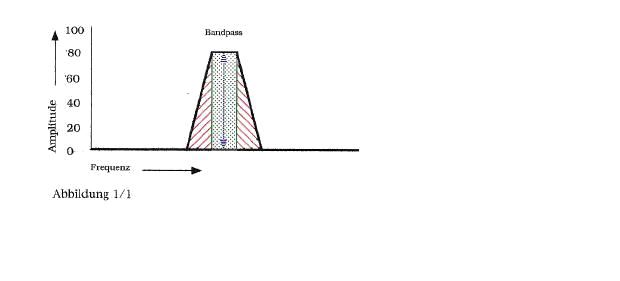
\includegraphics[width=1\textwidth]{images/nono/hph/ab_v_01.jpg}
\caption{}
\label{hph-img1}
\end{center}
\end{figure}

Mentre i due musicisti ed io abbiamo condotto i nostri esperimenti acustici, Luigi Nono deve aver aperto la porta del nostro studio e ascoltato gli esperimenti. All'improvviso entrò inaspettatamente, sorrise e disse: sono arrivato dopo tutto.
Poi ha annotato i risultati tecnici e sonori e come sono stati creati. Soprattutto Roberto ha dovuto mostrargli il suo nuovo flauto contrabbasso. Nono studiò i singoli campi di tono e suono, mise i suoi appunti nella sua borsa e disse: Devo tornare all'Halden-Hotel e continuare a lavorare. E quello stesso pomeriggio e sera, Luigi Nono ha composto le prime battute per "A Pierre", che ha provato, corretto e perfezionato con i musicisti e i tecnici dello Experimental Studio il giorno successivo.
Tornato a Venezia Nono finì immediatamente la versione finale di "A PIERRE", la prima esibizione avvenne pochi giorni dopo il 26 marzo 1985 a Baden-Baden, in occasione del 60 ° compleanno di Boulez.
Quindi, fate la genesi di Luigi Nonos A Pierre. Nono aveva studiato i nostri esperimenti sonori con molta attenzione e integrato nel suo nuovo lavoro in una forma completamente nuova. Il tempo di ritardo 12 e 24 secondi sono stati adottati da lui. Ha fatto uso del fatto che il suono della ripetizione filtrata e poco riverberata è andato ad estendere lo strato dopo 12 secondi.

\begin{figure}[htbp]
\begin{center}
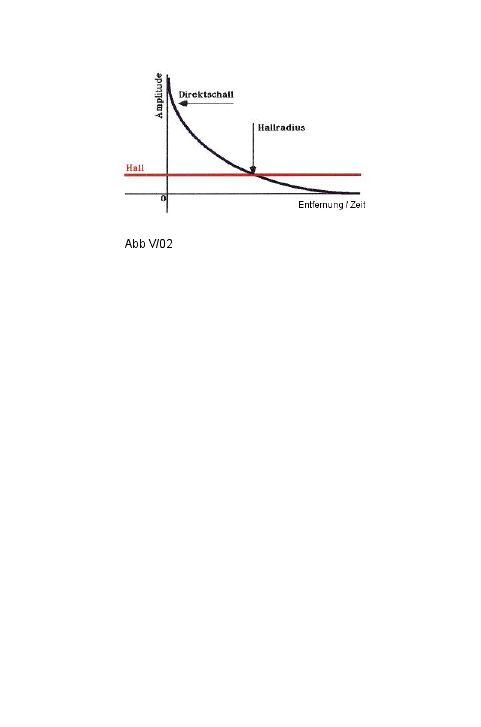
\includegraphics[width=1\textwidth]{images/nono/hph/ab_v_02.jpg}
\caption{}
\label{hph-img2}
\end{center}
\end{figure}

Conosciamo questo processo acustico come eco radiale, immagine 2. Con la diminuzione della dinamica del suono diretto e l'identica intensità del riverbero, percepiamo psicologicamente il suono diretto sempre più diffusamente in una distanza crescente. Questa estensione dello spazio sonoro diventa più chiara dalla trasformazione del suono diretto, dalla selezione del suono. Accanto al suono originale degli strumenti ci sono altri due livelli sonori, che sono enfatizzati dal loro ritardo di 12 e 24 secondi. Questa non è una dinamica, ma come accennato prima, un'estensione dello spazio dell'immagine sonora.
Nono sapeva dai nostri esperimenti a Friburgo, che questo poteva essere realizzato con un'idea musicale speciale e creato una forma di composizione strettamente orizzontale.

\begin{figure}[htbp]
\begin{center}
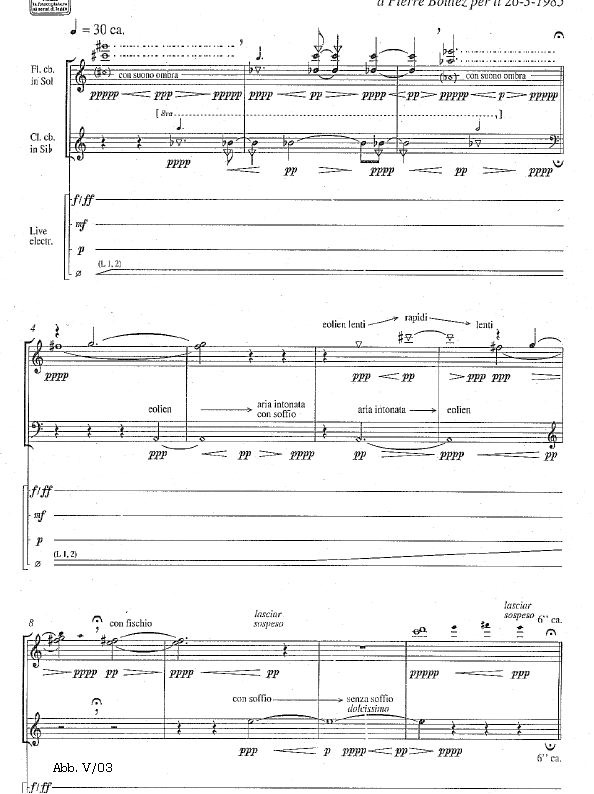
\includegraphics[width=1\textwidth]{images/nono/hph/ab_v_03.jpg}
\caption{}
\label{hph-img3}
\end{center}
\end{figure}


A prima vista, la partitura appare molto semplice, ma chiunque abbia studiato l'eccellente introduzione a A PIERRE nella Ricordi - avrà notato che Nono richiede per quasi ogni nota una forma di interpretazione individuale: dal fischio al fischietto. Per questo motivo, posso raccomandare lo studio di questi testi in tre lingue: italiano, inglese e tedesco.
Nono crea strutture sonore piene di contrasti che, secondo il tono, variano da suoni e toni pacifici ad aggressivi. Oltre a questo, il compositore ha utilizzato una trasformazione del suono per gli strumenti. Questa trasformazione - un piccolo sept e un tritone più basso - era guidata da un yy slow vibrato, che portava a un controllo variabile del pitch. Al fine di evitare un effetto sirena, questa trasposizione deve essere controllata molto dolcemente. Questa ricchezza di schemi sonori di entrambi gli strumenti suona insieme alla selezione del suono nei filtri passa banda e la trasformazione del suono crea nuovi spettri sonori molto interessanti, che - come mostrato nella figura 3 - possono essere ascoltati nella forma orizzontale di composizione di Nono in tutte le sottigliezze e vari livelli di suoni.
Certamente, Luigi Nono aveva già utilizzato materiali sonori simili per gli strumenti in "Amendes Klarsein" o in "Prometeo", ma insieme alla legenda tecnica finale come mostrato nel diagramma 4, il compositore realizza un'espressione musicale completamente nuova.

\begin{figure}[htbp]
\begin{center}
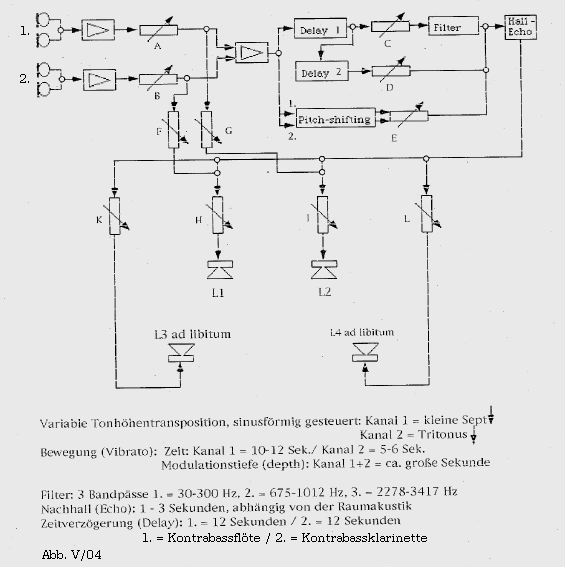
\includegraphics[width=1\textwidth]{images/nono/hph/ab_v_04.jpg}
\caption{}
\label{hph-img4}
\end{center}
\end{figure}

I singoli valori per il controllo dinamico e il tempo di riverbero sono indicati in percentuali relative e devono essere adattati all'acustica individuale della sala da concerto. La dinamica di Nono spazia da 5 pianissimos a forte, dove l'eruzione al forte appare solo una volta. Il più delle volte il volume varia attorno al pianissimo. Nono sviluppò ulteriormente la mia concezione di base dei miei esperimenti per evitare la ripetizione canonica udibile. Sulla base dei fermati a ripetizione continua di circa 6 secondi, la sequenza rigida di ripetizioni di 12 e 24 secondi si dissolve completamente. Così Nono impedisce una periodicità all'interno della sua musica che spesso si rivela molto differenziata e non ritmica, la cui forma interiore è composta in funzione del tempo. Pertanto, la direzione del suono deve essere così trasparente che l'ascoltatore non può verificare ciò che viene riprodotto in origine o ciò che viene riprodotto dagli altoparlanti. Due altoparlanti collocati dietro i solisti sono stati forniti per una performance. Successivamente, Nono collocò due altoparlanti aggiuntivi sul retro dell'auditorium, soprattutto nelle grandi sale da concerto, con la nota esplicita "ad libitum". Inoltre, il volume di questi 2 altoparlanti aggiuntivi 3 e 4 - dopo gli esperimenti con il compositore - deve essere controllato separatamente dagli altoparlanti 1 e 2. Il diagramma 5 mostra la relazione di dinamica tra gli altoparlanti.

\begin{figure}[htbp]
\begin{center}
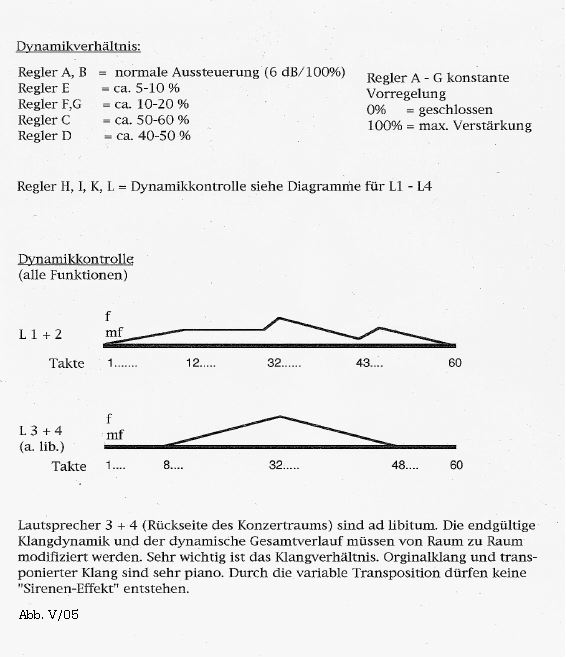
\includegraphics[width=1\textwidth]{images/nono/hph/ab_v_05.jpg}
\caption{}
\label{hph-img5}
\end{center}
\end{figure}

C'è stato il rimprovero che Live-Electronics, la trasformazione elettronica del suono sarebbe attributi di una composizione, che era stata aggiunta dopo il completamento del lavoro. Penso che non ci siano più composizioni tipiche di A Pierre e Omaggio a György Kurtag di Luigi Nono, che sconfiggono totalmente questo rimprovero. In entrambi i lavori, Nono ha incluso nel suo processo compositivo Live-Electronic come materiale equivalente accanto a strumenti meccanici tradizionali o voci. Entrambe le opere perderebbero la loro sostanza musicale senza l'estensione elettronica.
Lo sperimenteremo soprattutto nella recensione di Omaggio a György Kurtag. Per questo ora ho preparato un piccolo esempio con flauto solo. Innanzitutto, ascolterai un paio di battute da "A Pierre" senza Live-Electronics, quindi la stessa parte con estensione sonora elettronica:

Gli esempi sonori sono in mono. Il download completo è necessario prima dell'ascolto.

suono esempio 1 (Martin Fahlenbrock, flauto contrabbasso)
suono di esempio 2

Ci sono esempi che mostrano chiaramente che senza la transistor elettronica del suono, l'estensione del suono, uno strumento, manca una parte della sostanza compositiva. Come ho detto prima, dagli esperimenti di Freiburger, Nono sapeva esattamente i risultati sonori delle doppie ripetizioni, originali e trasformati. Ha composto le note degli strumenti con questo risultato, creando così una perfetta armonia tra meccanica e strumento elettronico. Non nego che ci siano composizioni, ad esempio Emmanuel Nunes: "Wandlungen", che può essere eseguita con e senza Live-Electronics. Tuttavia ciò non è possibile con le opere di Nonos create in collaborazione con Experimental Studio. Esigono un equilibrio tra i suoni degli strumenti tradizionali e i suoni della trasformazione elettronica. Di conseguenza non è possibile organizzare né nelle parti strumentali né nelle parti vocali e tecniche senza distruggere il suono che il compositore aveva puntato all'originale.

Ascoltiamo ora una sezione di "A Pierre" di Luigi Nono in una registrazione subito dopo il completamento della composizione, realizzata nel Freiburg Experimentalstudio (flauto di contrabbasso Roberto Fabbriciani e clarinetto contrabbasso Ciro Scarponi).

suono di esempio 3

\section{OMAGGIO A GYÖRGY KURTÁG}

La prima rappresentazione di "Omaggio a György Kurtág" il 10.6.83 a Firenze è stata una delusione per molti ascoltatori. È stata davvero una prima esibizione?
Nono stava lavorando a "Guai ai gelidi mostri" e "Prometeo" in quell'anno. Molte prove sperimentali hanno avuto luogo con la cantante Susanne Otto, lo strumentista Roberto Fabricciani, Ciro Scarponi e Giancarlo Schiaffini nello studio di Friburgo, una di queste prove è stato il concerto a Firenze. La composizione "Omaggio a György Kurtág" consisteva in valori soglia musicali, che Nono aveva indicato per ogni interprete in tono, spettri sonori e dinamici. Il compositore aveva anche dato alcuni suggerimenti per la tecnica della trasformazione del suono, che, tuttavia, non aveva nulla da fare con la versione finale di "Omaggio". Va detto che Luigi Nono, Alvise Vidolin e io - con la collaborazione dei musicisti - avevamo presentato una introduzione sulla trasformazione del suono elettronico all'inizio del concerto. Vorrei dire che la performance è stata un concerto di lavoro con il titolo: Composizione in corso. Nono non ha tratto profitto da questa esperienza in concerto fino alla sua composizione "Post-Prae-Ludium Donau" del 1987 per tuba solo e live-electronics. In questa composizione, per il musicista, valori di soglia, altezza, spettro sonoro, strutture ritmiche, scale di toni, volume e, soprattutto, sono state definite le strutture temporali. Gli intervalli devono essere riempiti dall'interprete mediante improvvisazioni. Sono indicati funzioni sonore e programmi per l'elettronica.
Quello che sto per dire ora si riferisce esclusivamente alla versione di "Omaggio", che è stata eseguita per la prima volta a Torino, il 6 giugno 1986.
All'inizio della mia conferenza scrissi: composizioni, in cui Luigi Nono aveva integrato in modo stringente una funzione estesa del tempo. Per A Pierre, Nono applica un ritardo di segnali acustici nel tempo, ripetizioni senza feedback. Sebbene questi determinino formalmente la composizione, l'idea di base di "Omaggio a György Kurtag" era completamente diversa.
Nono mi aveva comunicato il suo primo schizzo in una lettera:

\begin{figure}[htbp]
\begin{center}
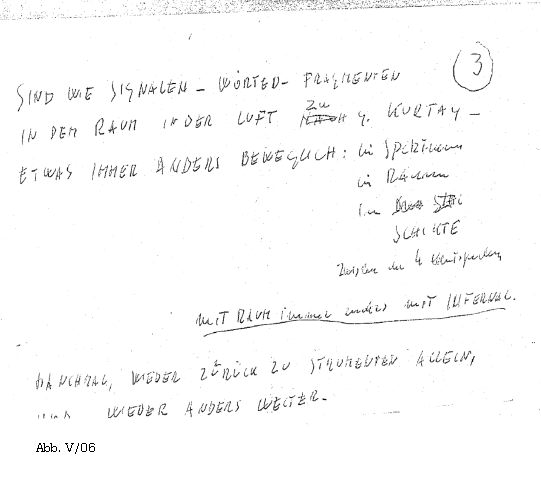
\includegraphics[width=1\textwidth]{images/nono/hph/ab_v_06.jpg}
\caption{}
\label{hph-img6}
\end{center}
\end{figure}

Cosa significa questo?
1.) La musica dovrebbe essere come segnali, parole, frammenti nell'aria, in
spazio a György Kurtag.
2.) Riguardo l'uso della trasformazione del suono elettronico Nono scrive:
Sempre nuovo, mai rigido, ma
cambio dello spettro, filtro passa banda,
cambiamento del suono dello spazio, varie posizioni del suono (4 altoparlanti), movimenti del suono, (esteso a 6 altoparlanti durante le prove),
La modifica del feedback significa feedback diverso al ritardo dei segnali.
3:) A volte solo strumenti, nient'altro che il suono strumentale e vocale originale.
4.) E ancora con live-electronics.
Per capire meglio, daremo un'occhiata alla foto 7, la leggenda tecnica, che ho registrato in questa forma durante le prove a Torino.

\begin{figure}[htbp]
\begin{center}
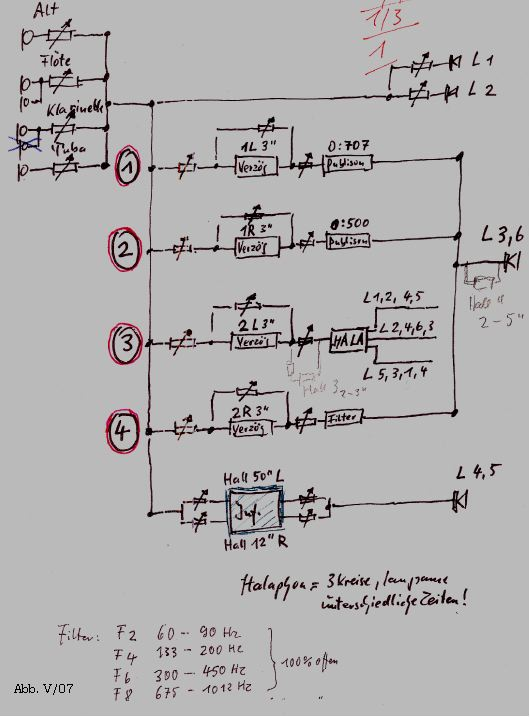
\includegraphics[width=1\textwidth]{images/nono/hph/ab_v_07.jpg}
\caption{}
\label{hph-img7}
\end{center}
\end{figure}

Per evitare equivoci, ho chiamato i programmi con combinazioni. Tutti e quattro sono ritardati di 3 secondi, con e senza feedback. A seconda della dinamica del feedback, i segnali di ingresso degli strumenti e la voce si attenuano in modo diverso. Al massimo una miscela di suoni nell'apparecchiatura di ritardo può essere memorizzata acusticamente per un periodo di tempo più lungo, alimentando le scale parzialmente orizzontali dei suoni originali sovrapposti, compressi e trasformati in una struttura verticale del suono. Nella sua lettera, Nono lo chiama: cambiamento nel feedback, che significa volume di feedback. Il cambiamento dello spettro sonoro - Nono non solo può ascoltarli durante le prove, ma anche vederli tridimensionalmente su uno schermo e battere con precisione - queste mutazioni sonore sono ottenute da tre possibilità:

1.) suddivisione dello spettro sonoro nei suoi singoli toni parziali. Conosciamo queste selezioni dalla prima ripetizione su A Pierre.
2.) Trasposizione di spettro in un harmonizer. Per "Omaggio" Nono ha scelto la trasposizione di un tritone e un'ottava più in basso. Mescolato con il suono originale, viene creato un nuovo spettro sonoro, dipendente dal volume di trasposizione.

Da un lato, lo spazio sonoro è cambiato da varie classi con i segnali di uscita ai 6 altoparlanti, dall'altro un movimento sonoro '150; ricorda alla combinazione tre. I movimenti sonori sono realizzati in tre diverse direzioni di movimento lente con un'apparecchiatura di controllo dello spazio sonoro universale, l'halaphone e sono definiti con precisione dal compositore. I singoli movimenti di direzione sono controllati tramite altoparlanti.
Fin dall'inizio, Luigi Nono ha avuto un'idea molto precisa dell'uso della trasformazione del suono elettronico per la sua composizione, che poi è stata resa più precisa durante le prove, Confrontiamo ancora una volta le figure 7 e 6.

Immagine 6

Immagine 7

Spectre - combinazione 4 , 5 filtri passa banda

spettro - combinazione 1 e 2 , trasformazione del suono

Combinazione 3- spazio - classificazione di altoparlanti, movimento del suono
Riverbero (12 + 50 secondi)

Feedback: ritardo di tre secondi con vari feedback

Corrispondente al suo schizzo tecnico, Nono ha composto la voce e la partitura strumentale:

Contrariamente a una forma prevalentemente verticale di Pierre, soprattutto alla realizzazione del lungo riverbero e dei suoni compressi dal feedback.

\begin{figure}[htbp]
\begin{center}
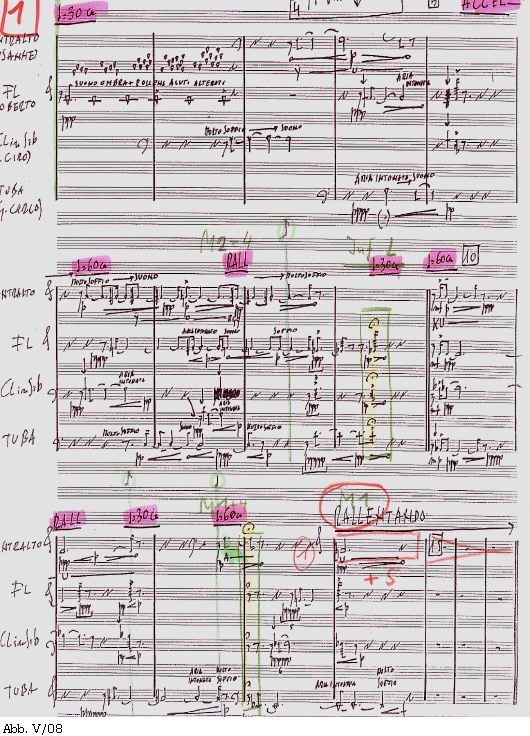
\includegraphics[width=1\textwidth]{images/nono/hph/ab_v_08.jpg}
\caption{}
\label{hph-img8}
\end{center}
\end{figure}

Nella figura 8 vediamo la prima pagina della partitura scritta a mano con note supplementari di controllo del suono, prima esecuzione, Torino. Nella barra 9, contrassegnata in verde, l'accordo dello strumento di ottone viene riverberato artificialmente per 50 secondi. Naturalmente, l'intensità di questo accordo - pianissimo - accorcia molto il riverbero. La durata del riverbero dipende dall'intensità del segnale di ingresso. Pertanto, Nono non indica una durata esatta, ma collega questo riverbero tecnicamente inesatto da un arresto. Ma ciò che può essere ascoltato, tuttavia, è il volume del suono, che corrisponde alla dimensione di una stanza geometrica di 50 secondi. Pertanto è importante che vengano utilizzate solo apparecchiature di ritardo con un volume di spazio controllato. La suddetta fermata consente al controllo del suono di variare in modo variabile attenuando il tempo di riverbero in base alle dimensioni della sala da concerto. Gli intervalli sonori realizzano lo schizzo di Nono. "come segnali a György Kurtag" Dove troviamo un intervallo sonoro più breve nella battuta 13, Nono impiega la prima versione di un intervallo sonoro di delay con feedback per il contralto nella barra da 14 a 17. Il tempo prescritto è un quarto di nota uguale a 60 , il tempo di ritardo con feed-back di 3 secondi. Con una mezza nota del contralto, si ottiene una ripetizione con un semplice feedback. La funzione di fadeout altrettanto breve del feedback è contrassegnata in rosso. Il suono originale della voce viene trasposto nel delay di un tritone in basso (combinazione 1).

\begin{figure}[htbp]
\begin{center}
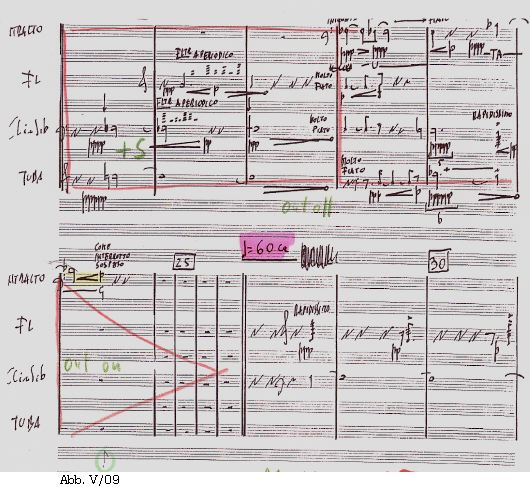
\includegraphics[width=1\textwidth]{images/nono/hph/ab_v_09.jpg}
\caption{}
\label{hph-img9}
\end{center}
\end{figure}

Nelle barre 18-20, Nono impiega la seconda versione dell'intervallo sonoro per ritardo con feedback. Tuttavia, vista formalmente, questa versione è completamente cambiata rispetto alla battuta 14. Il suono originale degli strumenti di ottone viene di nuovo ritardato di tre secondi con un feedback e una trasposizione di un tritone più in basso. Il risultato non può essere ascoltato immediatamente, ma viene riprodotto nella battuta 23 -27. Questo effetto acustico può essere chiamato eco con una lunga riverberazione, ovvero l'intensificazione del suono della barra 18-20 può essere percepita solo 20 secondi dopo. Un'idea compositiva, che combina due funzioni temporali in un unico complesso: durata della ripetizione con feedback e durata dell'eco. Nell'esempio 4, prima ascolteremo lo spazio sonoro ingrandito e il riverbero sovradimensionato.

suono di esempio 4

Il feedback è stato sbiadito. Nell'esempio seguente, ascolteremo un ritardo con feedback, formiamo uno senza cambiamenti nel tempo. Vorrei richiamare la tua attenzione sulla trasposizione in un tritone più in basso.

suono di esempio 5

La terza versione, il suono originale compresso e trasposto con riproduzione indietro spostato nel tempo. Il feedback si attenua lentamente, c'è un naturale sbiadimento dovuto alla dissoluzione della densità del suono. Questa procedura tecnica è particolarmente importante per una performance.

esempio sonoro 6

Questi esempi sonori sono continuamente modificati - come sappiamo dalla leggenda tecnica - durante l'intero lavoro. Così il compositore realizza il suo concetto: "Qualcosa è continuamente e diversamente flessibile"

La restante parte di voce e strumento rimane invariata senza la trasformazione del suono. Con questo, Luigi Nono enfatizza la funzione di live-electronic, gli intervalli sonori creano nuove dimensioni del suono e del tempo. Citazione del compositore: nello spazio cosmico verso l'universo, altri spazi, altre terre, altri abissi, altre fantasie. (Fine della citazione).
Con questi due lavori, "A Pierre" e "Omaggio a György Kurtág", Luigi Nono ha scoperto nuovi strati sonori, che ha potuto realizzare con l'aiuto della tecnica moderna, la trasformazione elettronica del suono. Sebbene diversi negli strumenti, diversi nella forma della composizione, entrambe le opere hanno un significato comune, un concetto spirituale comune.

Ascoltiamo "Omaggio a György Kurtag" due volte. Durante il primo replay, ti mostrerò il punteggio sullo schermo, per dimostrare cosa intendevo mostrare. prima. Poi ascolteremo il breve brano, circa 15 minuti, ascolteremo la musica di Nono, senza essere distratti dalle impressioni visive. Quest'opera di Nono è stata pubblicata in un'ottima edizione dalla casa editrice Ricordi. Sto usando una copia della partitura originale, poiché ho usato i colori per tutte le funzioni di live-electronic durante le prove per la prima esibizione a Torino.

Esempio 7 (con schermo)
Esempio 8 (senza schermo) Si prega di ascoltare gli esempi 7 e 8 dal CD "luigi nono 3", AUVIDIS FRANCE, MO 782047.
